%for reference to this section
\section{Introduction}
\label{section:Introduction}
text coming soon......

\section{Background and related work}
\label{section:RelatedWork}
Over the past 20 years, technology has evolved rapidly, and it has been incorporated into everyday life \autocite{sharmin2012effect, walker2000screen}. As a result, it is no surprise that schools and their teachers too want to combine traditional teaching methods with modern technology in the daily school life \autocite{lozano2016dedigitalizing}. However, when it comes to designing interfaces specifically for children, some difficulties arise, like \textcite{boyd2015evaluating, gan2015enhancing} are mentioning in their papers. Therefore, the following sections describe the most significant challenges and the leading points of previous approaches.

\subsection{Problem and Goals}
\label{subsection:ProblemGoals}
When creating a new interface, it is always essential to include the target audience in the designing process. This rule of thumb likewise applies to interfaces particularly fitted for children \autocite[]{gossen2012search, alhussayen2015evaluating}. As \textcite[]{gossen2012search, alhussayen2015evaluating} disclose in their papers, children experience and process their environment differently compared to adults. Depending on their present age, minors possess varying physical and more importantly varying cognitive skills. Therefore, an interface that is explicitly designed for adults may likely not fit the mind of a young child \autocite[]{alhussayen2015evaluating}.
Since children perceive the world differently in comparison to adults, various typographical distinctions and difficulties may arise as well \autocite{adattil2018effects}. For example, it is vital to use a bigger font size than usual as  \textcite{adattil2018effects} mention in their paper. Furthermore,  \textcite{adattil2018effects} recognized that reading time of regular texts decrease with age. 
Moreover, technology has changed a lot in the last few years as \textcite{liu2005reading} mention in their paper, however, technology is not entirely integrated into school life \autocite{engen2014ipads}. Nevertheless, many studies and projects like \textcite{walker2000screen, kerawalla2006making, engen2014ipads} have launched studies and projects to get children adapted to the usage of technology in schools and therefore, the normalization of digitizing education.

\subsection{Previous Approaches}
\label{subsection:PreviousApproaches}
As a result, different papers like \textcite[]{gossen2012search, alhussayen2015evaluating, lozano2016dedigitalizing} take different approaches to try to overcome that issue. 
For example, \textcite[]{gossen2012search} conducted a study with seven to 12-year-old students from Germany by introducing a newly designed search engine interface called "Knowledge Journey". This interface can be incorporated in class, specifically for information retrieval. The main renewal they introduced in their approach, in comparison to conventional search engines, is a guidance character that navigates through the whole search journey. The guiding figure offers the opportunity to support the child's search behavior, e.g., suggestions for new searches, handling wrong user input or any other possible failure while using the search engine \autocite[]{gossen2012search}.
Another approach has been tested by \textcite[]{alhussayen2015evaluating} in their study, where they presented their own learning platform called "Aseel Wa Raseel". While testing their interface, they found that children between the ages of seven and 12 years could not even fill out the registration form. As a result, they got remarkably frustrated with the program and hence could not fully use the platform in its intended utility. 
In contrast to the younger ones, most older children were able to complete the rather complicated registration process. Therefore, they could utilize the full range of features offered by their platform and proposed introducing a more gamified approach after testing the interface.




\section{Theoretical Part}
\label{section:TheoreticalPart}

\subsection{Definitions}
\label{subsection:Definitions}


\subsection{Health Literacy}
\label{subsection:HealthLiteracy}

\subsection{Technology and Education}
\label{subsection:TechnologyEducation}
Since technology has been going through an immense progression over the last two decades as \textcite{walker2000screen, liu2005reading} mention in their papers, humans have become more prone to integrate technology into everyday life. As a consequence, the education system also aims to incorporate technology into class as \textcite{walker2000screen, engen2014ipads, gan2015enhancing, lozano2016dedigitalizing, nouri2016teaching} disclose in their papers. \\
\subsubsection{Text-based Approaches}
One possibility to approach the objective to the digitization of education is the replacement of conventional reading material with digitized text supply \autocite{walker2000screen, liu2005reading, engen2014ipads}. 
\textcite{engen2014ipads} presented an iPad based application. It is a writing program, that reads the written text out loud every time the space bar is pressed and afterward, the sentence too when a child types a period. Moreover, \textcite{engen2014ipads} did a study on another application, that depicts the fairy tale red riding hood. Apart from the pictures on the iPad application, the text can either listen to an audio recording or read it out loud. Although the use of an iPad suggested uncomplicated handling, \textcite{engen2014ipads} observed that some children had troubles controlling the mobile devices while using the writing application. Hence, the use was not as intuitive as expected. 
Nevertheless, teachers still fairly welcomed the continuous usage of this iPad application in the classroom because it promotes the didactic skills of children \autocite{engen2014ipads}. 

\subsubsection{Interactive and Gamified Applications}
Another possible approach is the introduction of rather engaging and gamified applications as \textcite{gossen2012search, alhussayen2015evaluating, lozano2016dedigitalizing, gan2015enhancing} present in their papers. For example, \textcite{gossen2012search} created their own search engine interface called "Knowledge Journey" specially designed for children (see Figure \ref{figure:KnowledgeJourney}). 
\begin{figure}[!ht]
    \centering
    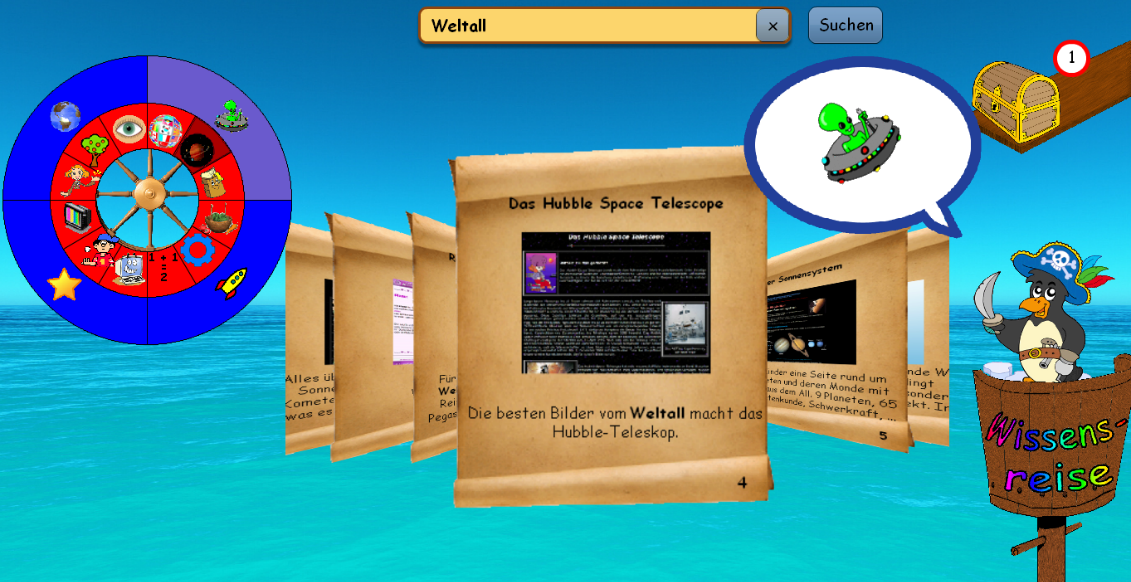
\includegraphics[width=1 \linewidth]{images/knowledge_journey.png}
    \caption{
        Screenshot of Knowledge Journey \autocite[60]{gossen2012search}
    }
    %for reference to this figure
    \label{figure:KnowledgeJourney}
\end{figure}
Their interface presents information, which can usually be retrieved with a conventional search engine, in a different way so that it is more inviting, interactable, and understandable for the minds of younger children. Furthermore, \textcite{gossen2012search} introduced a guidance character to handle possible failure and inexperience.
Another case was introduced by \textcite{alhussayen2015evaluating}, where they launched an arabic website called "Aseel Wa Raseel" that offers educational games for children. Although they used user-centered design in their development process, their platform disclosed some troubles for younger children. On their website, \textcite{alhussayen2015evaluating} included a rather long registration process, that prevented all younger children (seven to nine years old) and most of the older ones (10 to 12 years) to register on the website. 

\subsubsection{Augmented and Virtual Reality Applications}
Lastly, a rather innovative strategy is the implementation of augmented or virtual reality applications \autocite{saidin2015review, lozano2016dedigitalizing}. Based on this strategy, \textcite{kerawalla2006making}  analyzed different applications, including the solar system as the subject matter. These augmented reality applications were presented to children in elementary schools.
Although the children could create and manipulate the environment containing the planets, e.g., change size and rotation, it was mostly just animations to watch. Since the 3D animations did not require any further interaction, most children preferred simple role-play activities, where they could modify roles and interact with each other instead of only observe the 3D augmented animation \autocite{kerawalla2006making}.
Furthermore, \textcite{lozano2016dedigitalizing} introduced an educational game, that helps children build and refresh their knowledge of health literacy. With the help of tangible interfaces and mobile devices, \textcite{lozano2016dedigitalizing} succeeded to increase the motivation and satisfaction of the children. 
\textcite{saidin2015review} reviewed several different AR applications and concluded that AR has significant future potential, but still must be further developed. Most AR interfaces received positive feedback from the teacher side as well as from the student side. Especially the students proved to be more engaged with the learning process in schools \autocite{saidin2015review}.

\subsection{Why Children need different interfaces}
\label{subsection:ChildrenInterfaces}



\section{Practical Part}
\label{section:PracticalPart}
In the matter of this thesis, a study has been conducted to solidify all the findings in regards to interface design specifically made for children \autocite{gossen2012search, engen2014ipads, lozano2016dedigitalizing}. 
\\...\\

\subsection{Implementing the prototype}
\label{subsection:ImplementingPrototype}
For the implementation of this thesis, a React\footnote{https://reactjs.org/} project has been developed. As previous research from \textcite{gossen2012search, lozano2016dedigitalizing} showed, gamified approaches turned out to be more preferred by primary school children.
\\...\\

\subsection{Testing}
\label{subsection:Testing}

\begin{figure}[!ht]
    \centering
    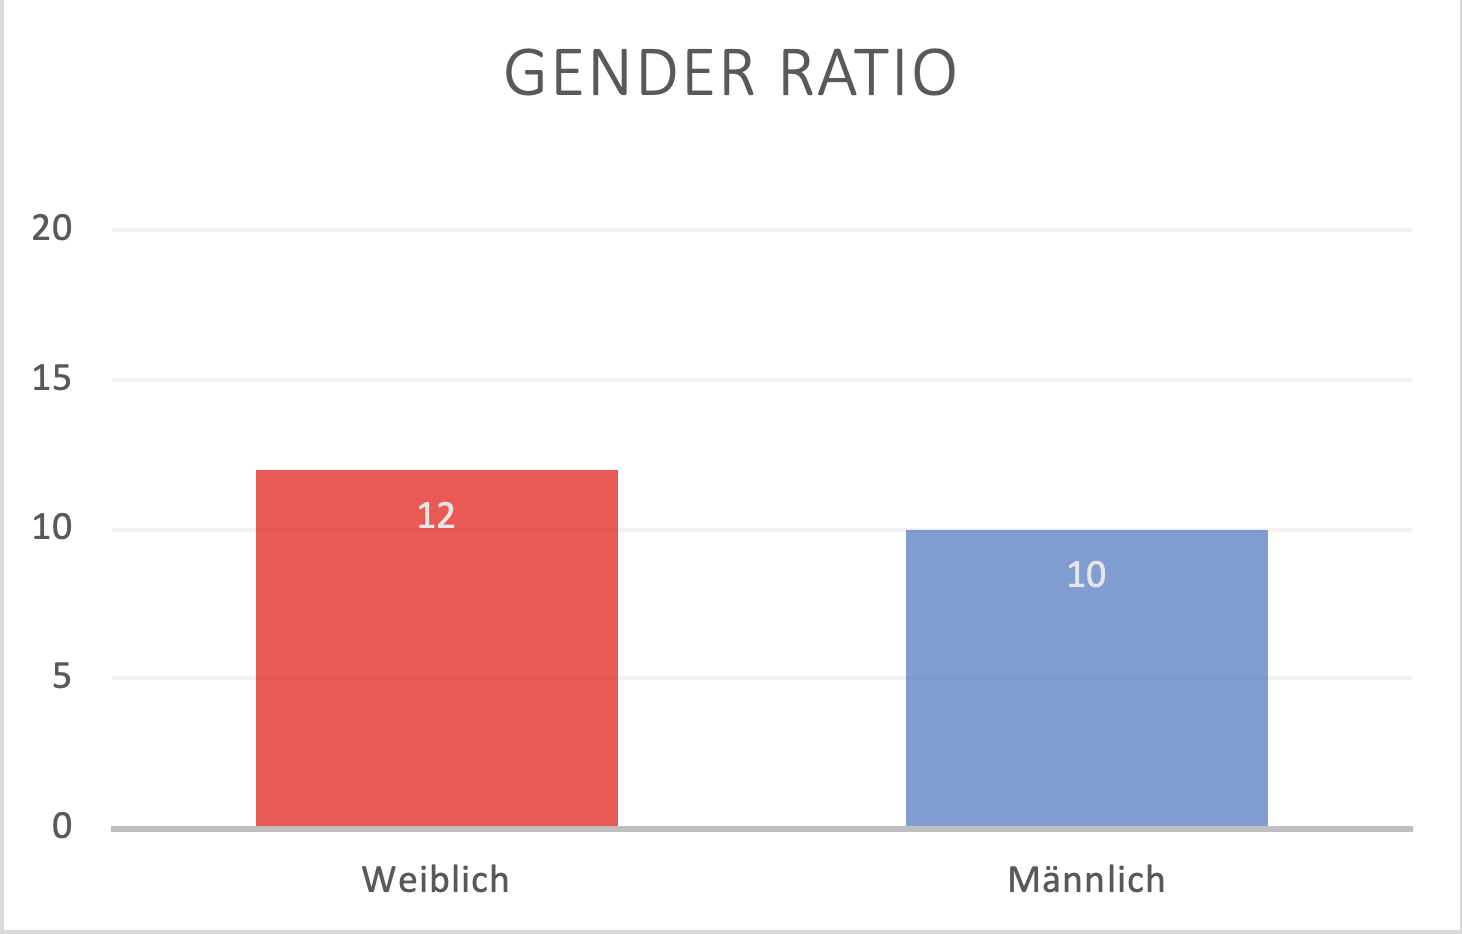
\includegraphics[width=1 \linewidth]{images/gender_ratio.png}
    \caption{
        Gender distribution between all children
    }
    %for reference to this figure
    \label{figure:GenderRatio}
\end{figure}

\begin{figure}[!ht]
    \centering
    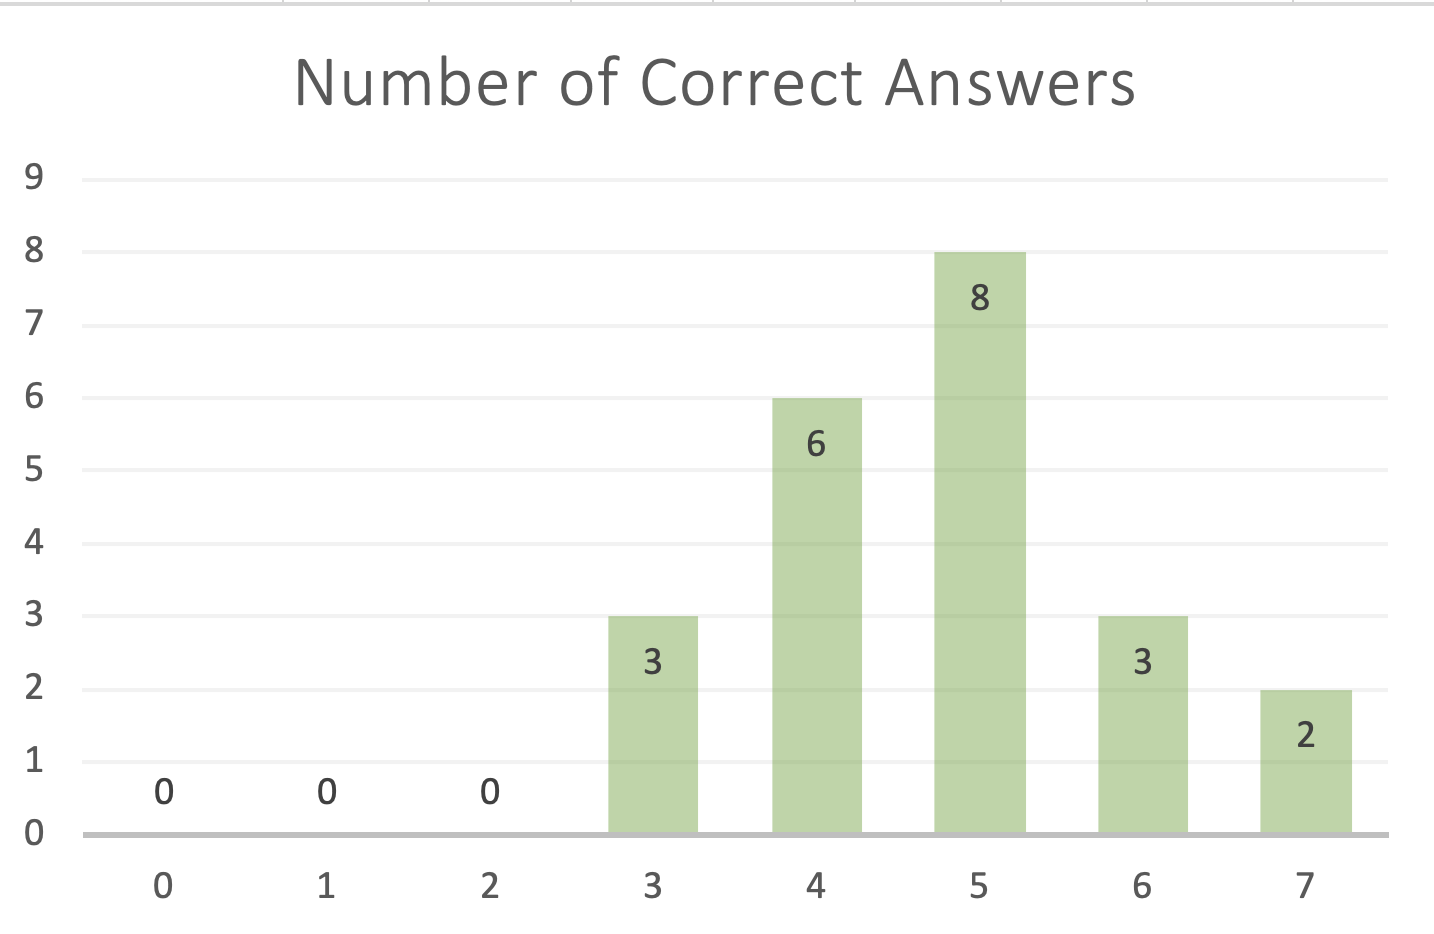
\includegraphics[width=1 \linewidth]{images/num_corr_answers.png}
    \caption{
        Distribution of correct given answers by all children
    }
    %for reference to this figure
    \label{figure:NummCorrAnswers}
\end{figure}

\subsection{Analyzing and evaluating the results}
\label{subsection:AnalyingResults}




\section{Discussion}
\label{section:Discussion}




\section{Conclusion}
\label{section:Conclusion}